\documentclass[a5paper,titlepage,10pt,openany]{scrbook}
\usepackage[a5paper,backref]{hyperref}
\usepackage[papersize={148.5mm,215mm},twoside,bindingoffset=0.5cm,hmargin={2cm,2cm},
				vmargin={2cm,2cm},footskip=1.1cm,driver=dvipdfm]{geometry}
\usepackage{palatino}
\usepackage[utf8]{inputenc}

\usepackage{pstricks}
\usepackage{graphicx}
\usepackage[bahasa]{babel} 
\usepackage{lettrine}
\usepackage{pifont}
\usepackage{enumitem}
\usepackage{wrapfig}
\usepackage{indentfirst}
\usepackage{parcolumns}
\usepackage[titles]{tocloft}
\usepackage{longtable}
\usepackage{microtype}
\usepackage{hyphenat}
%\usepackage[raggedright]{titlesec}
%\usepackage{titletoc}


\renewcommand{\cftchapfont}{%
  \fontsize{9}{8}\selectfont
}

\makeatletter
\renewcommand{\@pnumwidth}{1em} 
\renewcommand{\@tocrmarg}{1em}
\makeatother

\author{Lingkungan St. Petrus Maguwo}
\title{Warta Iman}
\setlength{\parindent}{1cm}
\psset{unit=1mm}


\begin{document}
\thispagestyle{empty}
\thispagestyle{empty}
\newcommand{\edisi}[1]{%
\DeclareFixedFont{\PT}{T1}{ppl}{b}{}{0.7in}
\DeclareFixedFont{\PTit}{T1}{ppl}{b}{it}{0.7in}
\DeclareFixedFont{\PTsmall}{T1}{ppl}{b}{it}{0.25in}
\DeclareFixedFont{\PTsmaller}{T1}{ppl}{b}{it}{0.175in}
\DeclareFixedFont{\PTsmallest}{T1}{ppl}{b}{it}{0.15in}

\begin{pspicture}(14cm,2cm)
\rput[rb](10.35cm,3cm){\PTsmallest {#1}}
\rput[lb](-2cm,1.5cm){\PT {WARTA IMAN}}
\rput[lb](0cm,0.5cm){\PTsmall {Lingkungan St. Petrus Maguwo}}
\end{pspicture}%
}

\newcounter{kgkcounter}[chapter]
\renewcommand{\thekgkcounter}{\arabic{kgkcounter}. }
\newcommand{\kgk}[1]{\refstepcounter{kgkcounter}\textbf{\flushleft \textbf{\thekgkcounter #1}}\\}

\newcommand{\kutipan}[1]{%
\noindent{\framebox{\parbox{10cm}{\centering\emph{#1}}}}}

\edisi{November 2011}

%\vspace{1cm}

\begin{center}
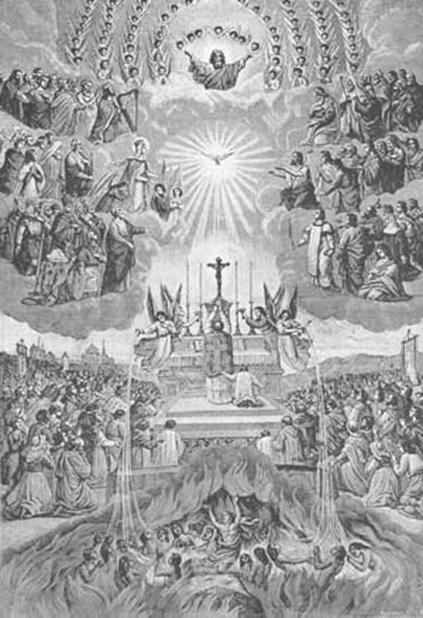
\includegraphics[scale=0.85]{gambar/purgatory2.jpg}
\end{center}

%\vspace{1cm}

\begin{center}
{\PTsmaller {Kasih, kerendahan hati, dan menurut pada kehendak Allah }}
\end{center}

\setlength{\parindent}{1cm}
\pagestyle{plain}
\chap{Sekilas Tentang Hari Raya Tubuh dan Darah Kristus}
 
Pesta \textit{Corpus Christi} (nama lengkapnya: \textit{Corpus et Sanguis Christi}), atau Hari Raya Tubuh dan Darah Kristus (dinamakan demikian kini), bisa ditelusuri asal-usulnya kembali ke abad ke-13.
Akan tetapi pesta ini merayakan sesuatu yang jauh lebih tua: institusi Sakramen Perjamuan Kudus di malam perjamuan terakhir.

Pada 1246, Uskup Robert de Thorete dari keuskupan Belgina dari Liège, atas saran biarawati Juliana dari Mont St Cornillon (juga di Belgia), mengadakan sinode dan melembagakan perayaan pesta ini.
Dari Liège, perayaan itu mulai menyebar, dan, pada September 8, 1264, Paus Urbanus IV menerbitkan buku kepausan “\textit{Transiturus de hoc mundo},” yang meresmikan Pesta Corpus Christi sebagai perayaan universal Gereja, yang akan dirayakan pada Kamis setelah Minggu Trinitas (minggu pertama setelah Pentakosta)

Atas permintaan Paus Urbanus IV, St Thomas Aquinas menulis ofisi (doa resmi Gereja) untuk pesta ini.
Ofisi ini secara luas dianggap salah satu yang paling indah di dalam \textit{Brevir} tradisional Roma (\textit{brevir} tradisional = buku doa resmi, Liturgi Jam Kudus), dan merupakan referensi himne Ekaristi terkenal “\textit{Pange Lingua Gloriosi}” (PS 502) dan “\textit{Tantum Ergo Sacramentum}” (PS 558 dan 559)

Selama berabad-abad setelah perayaan ini diperluas mencapai keseluruhan Gereja universal, perayaan itu juga dirayakan dengan prosesi ekaristi, di mana Hosti Kudus diarak ke penjuru kota, disertai dengan pujian dan litani. Sementara itu, umat beriman memuliakan Tubuh Kristus saat prosesi melewati mereka.

Beberapa kanon dari Kitab Hukum Kanonik yang memuat hari raya ini antara lain

\begin{description}
\item[Kan. 944 § 1] 	\textit{Jika menurut penilaian Uskup diosesan dapat dilaksanakan, sebagai kesaksian publik penghormatan terhadap Ekaristi mahakudus, hendaklah diselenggarakan prosesi lewat jalan-jalan umum, terutama pada hari raya Tubuh dan Darah Kristus.}
\item[Kan. 944 § 2] 	\textit{Uskup diosesan bertugas menetapkan peraturan-peraturan mengenai prosesi, dengannya dijamin partisipasi serta kepantasannya.}
\item[Kan. 1246 § 1] 	\textit{Hari Minggu, menurut tradisi apostolik, adalah hari dirayakannya misteri paskah, maka harus dipertahankan sebagai hari raya wajib primordial di seluruh Gereja. Begitu pula harus dipertahankan sebagai hari-hari wajib: hari Kelahiran Tuhan kita Yesus Kristus, Penampakan Tuhan, Kenaikan Tuhan, Tubuh dan Darah Kristus, Santa Perawan Maria Bunda Allah, Santa Perawan Maria dikandung tanpa noda dan Santa Perawan Maria diangkat ke surga, Santo Yusuf, Rasul Santo Petrus dan Paulus, dan akhirnya hari raya Semua Orang Kudus.}
\item[Kan. 1246 § 2] 	\textit{Namun Konferensi para Uskup dengan persetujuan sebelum- nya dari Takhta Apostolik, dapat menghapus beberapa dari antara hari- hari raya wajib itu atau memindahkan hari raya itu ke hari Minggu.}
\end{description}

Berdasar Kan 1246 point 2, di Indonesia Hari Raya Tubuh dan Darah Tuhan dirayakan pada Minggu kedua setelah Pentakosta. Untuk tahun 2012 ini jatuh pada tanggal 10 Juni 2012.




Secara tradisonal, pada awalnya sebutan yang tepat untuk Hari Raya Tubuh dan Darah Kristus adalah \textit{Sollemnitas Sanctissimi Corporis Christi}) yang kemudian dalam penggunaan populer digunakan frasa “\textit{Corpus Christi}”. Pada awalnya memang tidak ada kata “Darah” walaupun dalam teks Misa dan Ibadat Harian (\textit{brevir}) ada rujukan mengenai kata “Darah”



Perubahan yang terjadi adalah konsekuensi perubahan terhadap \textit{Festum Sanguinis Christi} (Pesta Darah Mulia). Pesta Darah Mulia adalah salah satu Pesta “devosional” terhadap kemanusiaan Kristus. (Dalam Gereja Katolik ada tiga tingkatan hari-hari istimewa, yaitu Hari Raya/\textit{Solemnitas}, Pesta/\textit{Festum}, dan Peringatan/\textit{Memoraria}). Pesta ini merupakan bagian dari “Pesta-pesta Sengsara” yang diadakan di hari-hari Jumat dalam Masa Prapaska di banyak tempat. 

 

Pada 1849, Paus Pius IX menyatakan hari Minggu pertama bulan Juli sebagai Pesta Darah Mulia dan wajib dirayakan secara universal. Namun demikian beliau tidak menghapuskan hari-hari Jumat “Pesta sengsara” yang masih dipraktikan pada berbagai penanggalan gerejawi lokal.

 

Ketika Paus Pius X melakukan pembaruan penanggalan liturgi, Pesta Darah Mulia dipindahkan menjadi tanggal 1 Juli, dan sejalan dengan kerangka liturgis yang ditetapkan pada hari itu, maka banyak keuskupan dan ordo tidak mempraktikan lagi “Pesta-pesta Sengsara”.Namun pesta-pesta ini tetap dipertahankan seperti yang tertulis pada appendiks buku pedoman misa (\textit{missal}) dengan judul “\textit{Pro Aliquibus Locis}” (di banyak tempat).

 

Pada 1961, semua pesta-pesta sengsara termasuk Pesta Darah Mulia yang tercantum dalam \textit{appendix}, dihapuskan, kecuali apabila ada permintaan dengan alasan yang masuk akal oleh ordo/kongregasi atau Keuskupan yang memiliki keterkaitan istimewa dengan pesta-pesta tersebut, misalnya kongregasi yang kemudian dikenal di Indonesia dengan nama Kongregasi Suster-suster Amalkasih Darah Mulia (ADM).

 

Kebijakan gerejawi berubah pada masa kepemimpinan Paus Yohanes XXIII. Beliau adalah seorang yang berdevosi pada Darah Mulia. Beliau menambahkan frasa “Terpujilah darahNya yang mahaindah” (PS No.205), mempromulgasikan (mengumumkan secara resmi) Litani Darah Mulia yang disertai dengan indulgensi, dan mempromosikan devosi terhadap Darah Mulia melalui ensiklik “\textit{Inde a Primis}”.

Pada tahun 1960-an ada perubahan penanggalan liturgi Gereja universal. Diputuskan bahwa pesta-pesta devosional harus dipindahkan atau paling tidak diturunkan tingkatannya. Pesta Darah Mulia yang dirayakan pada 1 Juli juga turut dihapuskan, walaupun tidak lama setelah keputusan ini dikeluarkan, banyak petisi dari para Uskup yang meminta agar Pesta Darah Mulia tetap dilestarikan. Namun demikian Konsili menolak petisi-petisi tersebut dan memutuskan untuk menambahkan kata “Darah” sehingga Hari Raya yang kita rayakan secara resmi hari ini dinamakan “\textbf{Hari Raya Tubuh dan Darah Kristus}” (\textit{Sollemnitas Sanctissimi Corporis et Sanguinis Christi}) atau boleh juga disebut “\textit{Corpus Sanguinisque Christi}”. Walaupun demikian, di banyak tempat, secara tradisional umat Katolik sudah telanjur terbiasa dengan penyebutan “\textit{Corpus Christi}” dan kita pun saat ini tetap boleh menyebut Hari Raya ini sebagai “\textit{Corpus Christi}” karena toh kita mengimani bahwa Hosti yang kita terima (apabila komuni hanya diterimakan dengan satu rupa), tidak pernah hanya Tubuh Kristus saja, melainkan sekaligus adalah Tubuh, Darah, Jiwa dan Keallahan Kristus, pendek kata SELURUH KRISTUS YANG TELAH WAFAT DAN BANGKIT, DAN KINI BERTAKHTA DI SISI BAPA. Hal ini sesuai juga dengan teks Kitab Suci, \textit{Jadi barangsiapa dengan cara yang tidak layak makan roti ATAU minum cawan Tuhan, ia berdosa terhadap Tubuh DAN Darah Tuhan..}(1 Kor 11:27)  .

 

Walaupun kita tidak lagi mempraktikkan Pesta Darah Mulia dalam penanggalan liturgi Gereja Universal, namun secara tradisional, Gereja Katolik mendedikasikan BULAN JULI demi penghormatan pada Darah Mulia Kristus.

\sumber{http://www.misa1962.org\\
http://www.facebook.com/notes/gereja-katolik}
\chap{Cara Menyambut Komuni}

Sebenarnya, jika kita mempelajari tradisi umum penerimaan Ekaristi, kita akan menemukan dua cara, langsung ke mulut atau di tangan. Memang, pada sampai sebelum Vatikan II, penerimaan Ekaristi dilakukan langsung ke mulut, namun pada tahun 1969, Roma mengeluarkan surat Instruksi yang memperbolehkan dua cara penerimaan Ekaristi, yaitu di tangan dan di mulut, dengan memberikan anjuran agar sedapat mungkin dipertahankan tradisi pemberian Ekaristi langsung ke mulut, walau tidak menutup kemungkinan pemberian ke tangan, jika itu diputuskan oleh konferensi para uskup di tempat yang bersangkutan, asal tetap menjaga penghayatan dan penghormatan yang layak kepada Ekaristi. Selengkapnya, silakan baca dokumen Instruksi resmi yang dikeluarkan oleh Paus Paulus VI, “\textit{Memoriale Domini“, the Instruction on the Manner of Administering Holy Communion, } \underline{The Congregation for Divine Worship on 29 Mei 1969}

Penerimaan Komuni langsung ke mulut dapat menghindari tercecernya serpihan-serpihan hosti yang kita percayai mengandung seluruh Kristus. Maka jika Komuni diberikan di tangan, maka perhatian khusus harus diberikan agar tidak ada serpihan hosti yang tercecer. Dan tak kalah penting, adalah tetap dengan hormat menerima Tubuh Kristus dengan sikap batin yang baik.

Dari segi kepraktisan, penerimaan komuni lewat mulut akan menghindari kemungkinan orang-orang yang ingin mendapatkan hosti untuk maksud-maksud yang tidak baik.

Penerimaan hosti (Sang Sabda yang menjadi daging) langsung ke mulut juga sesuai dengan ‘penerimaan Sabda Tuhan’ yang diberikan kepada nabi Yehezkiel(lih. Yeh 2:1,8,9,3: 1-3).

Mereka yang mendukung penerimaan Komuni di tangan, biasanya mengutip St. Sirilus/ Cyril (dari Yerusalem yang mengatakan, “Umat menerima Komuni dengan tangan kanan mendukung tangan kiri, dengan telapak yang membentuk cekungan; dan pada saat Tubuh Kristus diberikan, umat menjawab, Amen.” Atau juga St Basil (330-379) yang memperbolehkan pemberian Komuni di tangan pada jaman penindasan, yaitu pada saat tidak ada diakon/ imam yang dapat memberikan komuni.

Sebagai anggota Gereja Katolik di Indonesia, maka kita menghormati keputusan konferensi para uskup Indonesia, yang memperbolehkan penerimaan Ekaristi di tangan; walaupun sesungguhnya, kita dapat saja tetap menerima Ekaristi langsung di mulut, seperti yang dianjurkan oleh Bapa Paus. 

Di atas semua itu, perlu kita ingat, bahwa yang terpenting adalah penghayatan kita akan apa yang kita sambut; yaitu Kristus sendiri dalam rupa hosti. Cara penerimaan Komuni merupakan hal disiplin, yang jangan sampai mengaburkan makna Ekaristi itu sendiri. 

Seperti sudah pernah dibahas sebelumnya, maka terdapat dua cara menerima komuni, yaitu dengan tangan atau langsung di mulut/ di lidah.

Berikut ini adalah cara menerima komuni yang benar:

\subsubsection*{Dengan mulut/lidah}
\begin{enumerate}
\item        Berjalanlah ke hadapan Pastor/petugas Prodiakon dengan tangan terkatup.
\item        Sesaat sebelum giliran Anda menyambut Hosti, Anda maju dan tundukkanlah kepala anda dengan hormat untuk menghormati Kristus yang hadir dalam rupa Hosti kudus.
\item        Ketika Pastor/Prodiakon mengangkat hosti dan mengatakan “Tubuh Kristus”, pandanglah Hosti itu katakanlah “Amin” (artinya, Saya percaya)
\item        Bukalah mulut Anda dengan posisi lidah yang pantas agar Pastor/ petugas Prodiakon dapat meletakkan Hosti pada lidah Anda.
\item        Sambil Anda kembali ke tempat duduk Anda, Anda dapat mengunyah Hosti itu, ataupun membiarkan Hosti itu hancur di mulut Anda.
\end{enumerate}

\subsubsection*{Dengan Tangan}
\begin{enumerate}
\item        Berjalanlah ke hadapan Pastor/ petugas Prodiakon dengan tangan terkatup.
\item        Sesaat sebelum giliran Anda menyambut Hosti, Anda maju dan tundukkanlah kepala Anda dengan hormat untuk menghormati Kristus yang hadir dalam rupa Hosti kudus.
\item        Letakkan telapak tangan, satu di atas yang lain, dengan terbuka menghadap ke atas. Tangan yang dipakai untuk mengambil Hosti diletakkan di bawah telapak tangan yang lain.
\item        Arahkan telapak tangan Anda dengan jelas, sehingga Pastor/ Prodiakon dapat melihat bahwa Anda akan menerima Hosti dengan tangan.
\item        Ketika Pastor/ Prodiakon mengangkat hosti dan mengatakan “Tubuh Kristus”, pandanglah Hosti itu katakanlah “Amin” (artinya, Saya percaya)
\item        Setelah Hosti diberikan di telapak tangan yang teratas, ambillah Hosti tersebut dengan telapak tangan yang di bawah, dan segera letakkan hosti tersebut di mulut Anda. (Jangan membawa hosti tersebut ke bangku Anda/kemanapun)
\item        Sekembalinya Anda ke tempat duduk Anda, Anda dapat mengunyah Hosti itu, ataupun membiarkan Hosti itu hancur di mulut Anda.
\item        Pastikan Anda memakan serpihan Hosti (jika ada) yang mungkin jatuh di telapak tangan Anda.
\end{enumerate}

Menurut tata cara di atas, tidak ada ketentuan apakah tangan kiri atau tangan kanan yang di atas/ di bawah. Bagi kita orang Timur, memang jika kita menyambut dengan tangan, maka tangan yang mengambil Komuni ke dalam mulut adalah tangan kanan, tetapi ini tidak berarti bahwa harus demikian, karena orang yang kidal mungkin lebih dapat menggunakan tangan kiri.

Yang jelas jika sudah menyambut dengan tangan, jangan mengambil Hosti dengan lidah, karena resiko Hosti jatuh lebih besar. Kecuali jika Anda melihat ada serpihan Hosti di tangan, maka Anda harus mengambilnya dengan lidah Anda, untuk Anda makan. Sebab kita percaya serpihan Hosti itu juga adalah Kristus.

Jika ingin menyambut Hosti dengan mulut/lidah, silakan menyambutnya dengan cara yang benar.
\begin{center}
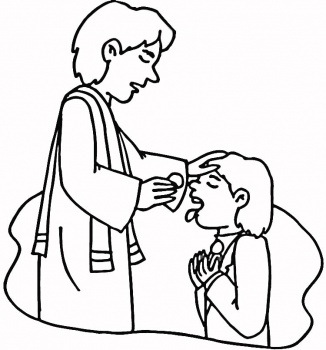
\includegraphics[scale=0.5]{gambar/communion-in-church-coloring-page.jpg}
\end{center}

\chap{Komuni Kudus dan Hidup Kita}


        Tema \textit{Warta Iman} (WI) kita bulan ini adalah KOMUNI. Istilah atau kata ini tentu  tidak asing di telinga kita. Barangkali makna dan pengaruhnya dalam hidup yang harus lebih kita dalami. Sebab untuk itulah  komuni lalu menjadi sebuah ``kata yang hidup'', sebuah kata yang memiliki realita konkrit dalam hidup  sehari-hari.

       Saya kira banyak dari kita paham bahwa komuni adalah salah satu  inti pokok dari liturgi ekaristi disamping doa syukur agung. Maksudnya ialah kalau ada suatu  liturgi tanpa melibatkan doa syukur agung dan komuni, maka liturgi itu tidak bisa disebut liturgi ekaristi. Kendati demikian agar inti pokok itu terlaksana dalam liturgi ekaristi maka persembahan atau persiapan roti dan anggur diperlukan dan ini menjadi sangat penting dan syarat mutlak, meskipun tidak menjadi bagian inti liturgi ekaristi. Sebab tidak mungkin ada komuni tanpa  roti dan anggur. Ketiga hal itu lalu secara bersama-sama  merupakan liturgi ekaristi.

      Namun demikian liturgi ekaristi sebagai inti perayaan ekaristi atau misa tidak berhenti di situ. Dalam tata ekaristi, liturgi sabda menjadi bagian penting dan diperlukan. Sebab di sana umat dipersiapkan untuk mengenang dan merenungkan karya keselamatan Allah dalam hidup, pewartaan dan karya Yesus dan terutama wafat dan kebangkitanNya. Dengan demikian umat kemudian bisa mengucap puji syukur kepada Allah sebagaimana itu menjadi inti pokok dari doa syukur agung. Oleh karena itu liturgi sabda benar-benar menjadi persiapan penting untuk liturgi ekaristi .

\section*{Pengaruh Komuni Dalam Hidup Kita}
      Dalam liturgi ekaristi ada tiga bagian pokok, tetapi dua di antaranya adalah inti liturgi ekaristi. Bagian pokok itu adalah persembahan, doa syukur agung dan komuni. Dua yang terakhir disebut inti liturgi ekaristi. Kendati persembahan tidak menjadi bagian dari inti liturgi ekaristi, namun persembahan menjadi syarat penting bahkan mutlak untuk terlaksananya liturgi ekaristi, sebab di dalam liturgi ekaristi dibutuhkan  roti dan anggur sebagai lambang yang pada hakekatnya mengandung makna dan nilai dari pemberian umat selain pemberian uang untuk keperluan Gereja dan kaum miskin. Persembahan lalu dimengerti sebagai pemberian umat bukan pertama-tama kepada Allah melainkan kepada Gereja yang kemudian oleh Gereja dipersembahkan atau dihunjukkan kepada Tuhan  di dalam liturgi ekaristi. Dalam arti inilah maka dalam perayaan ekaristi atau misa umat diperbolehkan  persembahan berupa hasil bumi misalnya padi, sayuran dan buah-buahan dls. Namun roti dan anggur tetap menjadi bahan penting untuk terlaksananya liturgi ekaristi. 

     Doa syukur agung dan komuni merupakan pusat dan puncak dari liturgi ekaristi (\textit{fons et culmen}). Atau dengan kata lain inilah inti liturgi ekaristi sebab di dalam doa syukur agung dan komuni itu iman Gereja diungkapkan secara resmi dalam doa puji syukur dan dalam doa pengudusan. Intinya adalah Gereja mengajak kita / umat bersyukur atas kebaikan Tuhan bukan saja kebaikan masa lampau tetapi terutama masa kini. Kita diajak bersyukur atas kekuatan Tuhan dan daya illahiNya, bersyukur atas keagungan dan kasihNya yang dinyatakan kepada kita. Bersyukur atas perlindungan dan jaminan Tuhan atas hidup kita dan atas kasihNya kepada kita yang tiada tara. Karena itu pantaslah kita  mengenang tanda kasih Allah itu teristimewa kasih Allah yang terbesar yaitu wafat Kristus (\textit{anamnese}) yang tentu juga atas kebangkitanNya yang mulia.

      Seluruh isi doa puji syukur sebagai ungkapan resmi iman Gereja, menjadikan kita dipersatukan dengan Kristus dan Allah oleh dan karena iman itu ketika kita mengenang wafat dan kebangkitanNya dan sekaligus dengan itu kita diperkenankan mengambil bagian di dalam pengharapan akan kebangkitan dan kehidupan abadi. Dan berkat iman Gereja juga dan oleh karya Roh Kudus, melalui doa pengudusan atas roti dan anggur kita dapat berjumpa dengan Kristus. Roti dan anggur berubah bukan sekedar menjadi tanda tetapi sungguh-sungguh Kristus hadir. Barangsiapa menyambut roti dan anggur itu dengan menyantapnya. ia menyambut kehadiran Kristus. Kristus hadir dalam hati orang yang menyambutNya Kristus hadir di dalam Gereja. Kristus hadir dalam setiap perayaan Gereja

      Maka komuni menjadi bagian inti liturgi yang penting. Sebab persatuan kita dengan Kristus terjadi ketika kita menyambut roti dan anggur yang telah dikuduskan dengan menyantapnya.  Melalui komuni sesuai dengan artinya (\textit{Communio}-kesatuan) maka kita dipersatukan dengan Kristus. Kita tinggal di dalam Kristus dan Kristus juga tinggal di dalam kita. Persatuan demikian menurut St. Yohanes akan menghasilkan buah. `` Barangsiapa tinggal di dalam Aku dan Aku tinggal di dalam dia, ia akan berbuah banyak'' (Yoh. 15: 4 -5) Maka setelah sekian kali -- mungkin ratusan kali -- kita menyambut komuni, sungguhkah kita telah menghasilkan buah ?

        Menurut Bapa Suci Benediktus XVI – dalam buku \textit{Paus Benediktus XVI, Sepuluh Gagasan Yang Mengubah Dunia}, Kanisius 2007 - ekaristi bila disikapi dengan sungguh-sungguh merupakan kekuatan yang luar biasa, kekuatan yang mampu mengubah dunia. Pada level pribadi kekuatan yang mampu mengubah dunia itu ialah iman ekaristi yaitu iman yang mendorong kita menjalani kehidupan menurut model Kristus. Apa yang telah kita santap (komuni) menjadikan hidup kita selaras dengan model Kristus itu (St. Augustinus). Dengan kata lain setiap orang yang dipimpin Roh karena persatuan kita dengan Kristus maka orang itu akan menghasilkan buah. Dan buah dari roh  menurut St. Paulus adalah kasih, sukacita, kebaikan, damai sejahtera, kesabaran, kemurahan, kesetiaan, kelemahlembutan, penguasaan diri (Gal. 5: 22) Dan kasih sendiri adalah sabar, murah hati, tidak sombong, tidak egois, tidak dendam, tidak iri hati (cemburu) (1 Kor. 13:4-5) Inilah beberapa  bagian dari hidup menurut model Kristus  

        Tentu bagi kita iman ekaristi bahwa persatuan kita dengan Kristus terjadi melalui komuni kudus selayaknya terus menerus kita renungkan: apakah kita memang telah dan sedang mengalami perubahan atau pembaharuan hidup karena sering menyambut komuni kudus? Katakanlah dalam kehidupan sehari-hari,  yang semula kita suka marah-marah misalnya kini menjadi lebih sabar, lebih mampu mengontrol emosi. Mampu mengusai diri dari kecenderungan-kecenderungan berbuat buruk, tidak lagi gemar membicarakan keburukan orang lain ``\textit{nggrenengi}'', menjadi bijaksana dalam bicara terutama menyangkut orang lain dan keburukannya. Tindakan-tindakan kebaikan yang didasari kasih makin menonjol.  Dalam kehidupan religius secara pribadi,  makin kentara mulai mempunyai kebiasaan melakukan doa pribadi atau perenungan sabda Tuhan (membaca Kitab Suci), rindu untuk selalu ikut perayaan ekaristi atau kegiatan olah rohani lainnya. Tentu kita masih bisa menggali lebih dalam.

         Dalam suatu riset yang diterbitkan oleh seorang professor dari Universitas Virginia Bradford Wilcox dan polling yang dilakukan oleh Gallup sebuah organisasi riset di Amerika menyimpulkan bahwa orang yang rajin mengikuti kebaktian terutama para pria Amerika hidupnya akan lebih bahagia. Pernikahannya bila pria itu sudah menikah, ia lebih bertanggung jawab terhadap pendidikan anak dan tidak suka melakukan kekerasan fisik terhadap anak maupun isteri. Orang juga memiliki emosi positip dari pada orang yang tak pernah datang ke Gereja yaitu bisa menikmati hidup, segar dan murah senyum serta suka melakukan sesuatu yang menarik dalam kebaikan.(http://www.jawaban.com)

Riset ini sebetulnya bukan sesuatu yang baru berkaitan dengan iman ekaristi, namun toh bisa memberikan gambaran yang sama bahwa kebiasaan menyambut tubuh dan darah Kristus (komuni) secara personal seharusnya makin mengubah hidup kita, hidup yang diperbaharui.

       Pada level sosial, iman ekaristi, persatuan kita dengan Kristus mendorong kita melakukan usaha-usaha membangun suatu dunia atau masyarakat di mana kasih Kristus yang selalu diperbaharui pada waktu ekaristi,  menjadi landasan bagi masyarakat yang dibangun itu sekalipun  terpaksa berlawanan dengan ideologi, keuntungan atau kehendak buta akan kekuasaan. Bapa Paus mengingatkan kita betapa pentingnya kasih yang ditimba dari kasih Kristus menjadi landasan dalam usaha-usaha membangun kehidupan bersama termasuk keluarga dan linkungan kita St. Petrus.  Bila hal itu terus bergerak dari kehidupan bersama yang satu ke kehidupan bersama yang lain, maka dunia akan sungguh berubah  Menurut St. Yohanes ``Inilah kemenangan yang mengalahkan dunia, iman kita `` (1 Yoh. 5:4) Tentu saja usaha-usaha demikian tidak mudah, sebab harus mengadapi berbagai tantang yang tidak ingin dunia berubah.

       Bagaimana dengan kehidupan bersama kita terutama keluarga dan lingkungan St. Petrus? Tentu saja bila kita sebagai pribadi senantiasa menyambut komuni, kita percaya  kasih Kristus akan makin kentara dalam usaha-usaha yang kita lakukan demi dan untuk keluarga dan lingkungan kita.yang lebih baik. Ledakan kebaikan dari pemecahan nuklir inti terdalam makhluk yaitu kemenangan kasih atas kebencian dan kematian, sedikit demi sedikit akan memicu rangkaian perubahan lain  menuju dunia yang lebih baik – demikian Bapa Paus menggambarkan kekuatan kasih Kristus yang senantiasa disegarkan dalam perayaan ekaristi bagi kehidupan bersama.

\section*{Hidup Subur}
      Akhirnya kita tahu bahwa buah-buah kehidupan itu muncul dari hidup yang subur. Hidup yang berasal dari penyerahan diri kita kepada Allah, sebagai jawaban atas undangan Kristus kepada kita ``Tinggallah di dalam Aku, dan Aku di dalam kamu'' (Yoh. 15:4) Inilah kehidupan rohani kita. Akan tetapi kehidupan rohani itu tidak dengan sendirinya menghasilkan buah bila tidak dipupuk dengan kasih mesra. Itulah sebabnya mengapa St. Yohanes berbicara mengenai iman dan kasih itu memiliki kaitan erat bahkan azasi. Karena iman kepada Allah dalam Roh Yesus, kita menerima Allah sebagai Bapa (1 Yoh.4:26) dan karena itu kita harus melakukan perintah-perintahNya. Perintah itu ialah mengasihi Allah (Mrk. 12:30). Akan tetapi kasih kepada Allah itu membutuhkan ungkapan dan ungkapan itu nyata dalam kasih kita kepada sesama.

\small
       Bila Yohanes Pembaptis berbicara keras tentang pohon  yang tidak berbuah ditebang dan dibuang ke dalam api  (Mat. 3:10) itu mengingatkan kita akan arti penting hidup rohani kita. Sebab hidup rohani yang tidak berbuah adalah hidup rohani yang mandul. Tentu bagi kita sangat tidak nyaman atau enak disebut sebagai orang mandul. Barangkali yang lebih menyakitkan kalau kita disebut orang katolik yang tidak menghasilkan buah kakatolikkannya, sekalipun setiap hari kita menyambut komuni. Untuk itu marilah merenungkan prinsip-prinsip dasar hidup seorang yang memiliki hidup subur sebagai penutup tulisan ini. Ada 3 segi kehidupan yang subur  menurut Henri JM. Nouwen dalam bukunya ``\textit{Tanda-Tanda Kehidupan}'':

\begin{enumerate}
\item Hidup yang subur adalah hidup yang tidak menutup diri dengan segala pertahanan diri, melainkan hidup yang terbuka terhadap kelemahan sekalipun rawan terhadap luka hidup. Yesus Kristus menjadi pola hidup subur yaitu hidup ``terbuka mudah kena''(\textit{vulnerability}) bahwa sekalipun Allah, Ia tidak mengganggap kesetaraanNya itu sebagai milik yang harus dipertahankan, tetapi justru mengosongkan diriNya sendiri dan menjadi sama dengan manusia (Flp. 2: 6 – 7)
\item Hidup yang subur adalah hidup yang penuh syukur. Syukur yang mengalir dari anugerah Tuhan yang Ia berikan dalam kasih dengan cuma-cuma kepada kita sebagai anugerah dan kita bagirasakan kepada saudara-saudara kita. Dalam kisah pergandaan roti (Yoh. 6 : 5-15) kita melihat bagaimana Yesus memberi contoh menghayati hidup subur. Setelah mengucapkan syukur atas 5 roti dan 2 ikan, Ia menyuruh para murid membagikannya kepada orang banyak. Membagikan kebaikan karena kebaikan hati Allah adalah ciri hidup subur.
\item Hidup subur adalah hidup yang dipelihara dan diperhatikan. Buah kehidupan tidak  muncul dengan sendirinya tanpa ada pemeliharaan dan perhatiaan.Yesus memberikan  contoh kepada kita bagaimana Ia memberikan perhatian kepada orang-orang yang Ia jumpai tanpa memaksa atau mengusai, melainkan melalui sabda dan tindakanNya Ia menawarkan kesempatan kepada mereka untuk mencari arah hidup dan keputusan-keputusan yang baru.
\end{enumerate}

\sumber{Yogyakarta, 17 Mei 2012\\
Hari Kenaikan Tuhan Yesus Ke Surga\\
(AS)}
\normalsize
\chap{Percayakah  Anda dengan Mukjizat Ekaristi?}
\small
    Barangkali kita masih ingat kabar tentang hosti suci berubah menjadi tetes noda darah di lantai ketika hosti jatuh dari tangan seorang umat yang menyambutnya di Paroki Kota Baru.  Kabar itu segera menyebar ke kalangan umat dan menimbulkan pertanyaan:  benarkah demikian ? Tentu bagi orang yang tidak percaya tidak mungkin bisa diberi penjelasan. Sebaliknya bagi orang yang percaya tidak diperlukan lagi penjelasan.

    Di bawah ini saya ingin menyampaikan kisah-kisah mukjizat ekaristi ``Miracles of the Eucharisti''; The Eucharisti Apostles of The Divine Mercy; www.thedivinemercy.org sebagaimana diterjemahkan YESAYA : www.indocell.net/yesaya.Sebetulnya ada 21 kisah, akan tapi tentu tidak semua bisa di coba di sini atau disajikan. Saya akan mengambil beberapa saja. Mudah-mudahan bisa berguna bagi peneguhan kehidupan rohani kita khususnya terhadap Ekaristi.
\normalsize
 

\renewcommand{\thesection}{\arabic{section}.}

\section{ALATRI, tahun 1228}

Seorang pemudi, yang tertarik pada seorang pemuda, diminta untuk membawa sekeping Hosti yang telah dikonsekrir agar dapat dibuatkan ramuan cinta. Sang pemudi menerima Komuni dan berjalan pulang ke rumah, tetapi karena merasa bersalah ia menyembunyikan Kristus di suatu pojok rumah.

Beberapa hari kemudian, ia datang dan mendapati bahwa Hosti telah berubah warna seperti daging. Imam paroki segera diberitahu dan ia membawa Hosti kepada Uskup. Bapa Uskup menulis surat kepada Paus Gregorius IX yang isinya:
\small
\qti{``Kita patut menyampaikan puji syukur sedalam-dalamnya kepada Dia yang, sementara senantiasa menyelenggarakan segala karya-Nya dengan cara-cara yang mengagumkan, pada kesempatan-kesempatan tertentu juga mengadakan mukjizat-mukjizat dan melakukan hal-hal menakjubkan agar para pendosa menyesali dosa-dosa mereka, mempertobatkan yang jahat, dan mematahkan kuasa bidaah sesat dengan memperteguh iman Gereja Katolik, menopang pengharapan-pengharapannya serta mendorong amal kasihnya.     
\\{~}\\
Oleh sebab itu, saudaraku terkasih, dengan surat Apostolik ini, kami menyarankan agar engkau memberikan penitensi yang lebih ringan kepada gadis tersebut, yang menurut pendapat kami, dalam melakukan dosa yang teramat serius itu, lebih terdorong oleh kelemahan daripada kejahatan, terutama dengan mempertimbangkan kenyataan bahwa ia sungguh menyesal setulus hati ketika mengakukan dosanya. Namun demikian, terhadap wanita yang menghasutnya, yang dengan kejahatannya mendorong si gadis untuk melakukan dosa sakrilegi, perlu dikenakan hukuman disipliner yang menurutmu lebih pantas; juga memerintahkannya untuk mengunjungi semua Uskup di wilayah terdekat, guna mengakukan dosa-dosanya kepada mereka dan mohon pengampunan dengan ketaatan yang tulus \ldots''
}
\normalsize

Mukjizat Hosti dipertontonkan dua kali setahun, yaitu pada hari Minggu pertama sesudah Paskah dan hari Minggu pertama sesudah Pentakosta.

Pada tahun 1960, Uskup Facchini dari  Alatri membuka segel tempat Hosti disimpan dan mengeluarkannya. Uskup menyatakan bahwa Hosti tetap dalam keadaan sama seperti saat pertama diketemukan, yaitu, sekerat daging yang tampak sedikit kecoklatan.

Pada tahun 1978, perayaan-perayaan istimewa diselenggarakan untuk memperingati 750 tahun terjadinya mukjizat.

\textit{``Akulah roti hidup. Nenek moyangmu telah makan manna di padang gurun dan mereka telah mati. Inilah roti yang turun dari sorga: Barangsiapa makan dari padanya, ia tidak akan mati.'' (Yoh 6:48-50)}
 

\section{ORVIETO dan BOLSENA, tahun 1263}

Mukjizat ini terjadi pada masa suatu ajaran sesat yang disebut Berengarianisme merajalela di Eropa. Bidaah ini menyangkal Kehadiran Nyata Kristus dalam Ekaristi. Pada tahun 1263, seorang imam bernama Petrus dari Prague sedang dalam perjalanan ziarah ke Roma untuk berdoa di makam pelindungnya, St Petrus, sebab ia menghadapi masalah yang amat serius. Ia merasakan kebimbangan yang besar mengenai Kehadiran Nyata Yesus dalam Ekaristi Kudus. Ia berdoa agar santo pelindungnya memohonkan rahmat baginya guna menyelamatkan imannya yang goyah. Dalam perjalanan, ia singgah untuk bermalam di suatu kota kecil bernama Bolsena, sekitar 70 mil sebelah utara Roma.

Keesokan harinya, Pastor Petrus merayakan Misa Kudus di Gereja St Kristina. Sementara ia mengucapkan kata-kata konsekrasi, “Inilah TubuhKu,” roti di tangannya berubah rupa menjadi Daging dan mulai mencucurkan darah dengan derasnya. Darah jatuh menetes ke korporal. Pastor Petrus amat terperanjat; ia tidak tahu apa yang harus diperbuatnya. Maka, ia membungkus Hosti Kudus dalam Korporal lalu pergi meninggalkan altar. Sementara ia berjalan pergi, tetesan-tetesan Darah jatuh ke atas lantai pualam di altar.

Paus Urbanus IV sedang berada di kota Orvieto, yang tak jauh dari sana. Pastor Petrus segera menemui paus guna menceritakan apa yang telah terjadi. Paus segera mengutus seorang uskup ke Gereja St Kristina guna menyelidiki peristiwa tersebut dan mengambil Korporal.

Segera sesudah Paus menerima Korporal dari Uskup, ia pergi ke balkon Istana Kepausan dan dengan hormat mempertontonkan mukjizat Korporal kepada orang banyak. Bapa Suci menyatakan bahwa mukjizat Ekaristi telah terjadi guna mengusir bidaah Berengarianisme. Pada saat yang sama, seorang pengikut St. Yuliana dari Liège menghubungi paus untuk sekali lagi memohon demi ditetapkannya Hari Raya Corpus Christi. Setahun kemudian, pada tahun 1264, Paus Urbanus IV memaklumkan Hari Raya agung ini kepada seluruh Gereja. (Mukjizat Korporal disimpan hingga kini di Katedral Orvieto. Lantai pualam bernoda Darah disimpan di Gereja St Kristina di Bolsena).  

\section{CASCIA, sekitar tahun 1300}
Cascia adalah sebuah kota kecil di pegunungan di lembah Umbrian, Italia. Itulah kota kediaman St. Rita dari Cascia. Jenazah St. Rita yang hingga kini masih utuh dibaringkan di Basilika Utama. Di bawahnya, di Basilika Kecil, disimpan Mukjizat Ekaristi dan jenazah Beato Simone Fidati, seorang imam yang terlibat langsung dalam mukjizat tersebut.

Pada masa terjadinya mukjizat, seorang imam tak lagi memiliki rasa hormat terhadap Ekaristi. Ketika diminta untuk mengantarkan Sakramen Mahakudus kepada seorang petani yang sedang sakit, ia mengambil sekeping Hosti yang telah dikonsekrasikan, menempatkannya dengan sembarangan di antara halaman-halaman buku breviary, lalu berangkat. Ketika ia membuka bukunya, ia mendapati bahwa Hosti telah berubah warna merah darah segar dan darah meresap ke kedua halaman buku di mana Hosti diselipkan.

Imam tersebut kemudian mohon nasehat Beato Simone Fidati, seorang imam yang kudus dan dihormati pada masa itu. Pastor Fidati menerima pengakuan sang imam dan memberinya absolusi. Beato Fidati mengambil kedua halaman dari breviary itu; satu ditempatkannya di tabernakel di Perugia dan satunya lagi ditempatkannya di Cascia. Mukjizat Ekaristi ini diperingati secara istimewa di Cascia setiap tahun pada Hari Raya Tubuh dan Darah Kristus.

Orang-orang yang melihat ke halaman yang ternoda darah itu dapat melihat gambar Kristus tertera di sana.

Ya Kristus, berilah kami rahmat agar dapat melihat Engkau dalam Ekaristi dan mengenali-Mu pada saat pemecahan roti.

 

\section{BAGNO DI ROMAGNA, tahun 1412}
Mukjizat Ekaristi ini terjadi di sebuah kota kecil di Italia bernama Bagno di Romagna ketika seorang imam merayakan Misa dengan dihantui keragu-raguan yang besar akan Kehadiran Nyata Kristus dalam Ekaristi. Setelah mengkonsekrasikan anggur, imam melihat ke dalam piala dan amat terkejut melihat bahwa anggur telah berubah menjadi darah. Darah mulai meluap keluar dari piala dan membasahi korporal. Terguncang oleh peristiwa adikodrati ini, imam segera berdoa mohon pengampunan. Kelak, ia bahkan digelari Venerabilis karena kesalehan hidupnya setelah terjadinya mukjizat.

Pada tahun 1912, ulang tahun ke-500 mukjizat Ekaristi, suatu perayaan besar diselenggarakan. Pada tahun 1958, dilakukan penelitian ilmiah yang hasilnya menguatkan bahwa darah di korporal adalah darah manusia dan masih mengandung karakteristik darah setelah hampir 600 tahun sesudah mukjizat terjadi.

Mungkin mukjizat Darah yang meluap hendak menunjukkan kepada kita bahwa Yesus sungguh hadir dalam Ekaristi. Mari merenungkan bagaimana seharusnya kita berubah setelah menyambut Yesus dengan mengijinkan-Nya tinggal dalam kita dan mengisi kita dengan kuasa Roh Kudus.

\section{MIDDLEBURG ~ LOUVAIN, tahun 1374}
Pada tahun 1374, seorang pemuda dengan dosa berat dalam jiwanya pergi menyambut Komuni Kudus. Ketika Hosti ditempatkan di atas lidahnya, Hosti berubah menjadi Daging sehingga ia tak dapat menelannya. Darah menetes dari bibirnya dan membasahi kain pada rel komuni. Imam bertindak cepat dengan mengambil Hosti Kudus serta menempatkannya dalam sebuah piala di altar.

Berita mengenai mukjizat ini tersebar keseluruh penjuru Belgia dan mukjizat Hosti dipindahkan 700 mil jauhnya ke Cologne. Sebuah ostensorium berhias indah dibuat. Sebagian Hosti dan sepotong kain dengan noda darah kemudian dibawa ke Louvain di mana telah dipersiapkan sebuah wadah reliqui yang indah.

Bagian mukjizat Ekaristi yang disimpan di Louvain berwarna agak kecoklatan dan dapat dikenali dengan mudah sebagai daging. Reliqui disimpan dalam sebuah wadah reliqui yang dibuat pada tahun 1803. Dokumen-dokumen penting dan hasil penelitian terhadap reliqui disimpan dalam perpustakaan Gereja St. Jacques.

\section{BOLOGNA, tahun 1333}
Mukjizat ini terjadi pada tahun 1333 di Bologna, Italia karena seorang gadis remaja saleh yang berumur sebelas tahun memiliki kerinduan yang berkobar-kobar untuk menyambut Kristus dalam Ekaristi.

Imelda Lambertini dilahirkan dalam sebuah keluarga kaya. Ayahnya adalah Count Eagno Lambertini. Imelda bergabung dalam Biara Dominikan ketika usianya baru sembilan tahun. Ia disayangi oleh para biarawati lainnya. Dalam usia yang masih sangat muda, Imelda memiliki cinta yang menyala-nyala kepada Yesus dalam Ekaristi dan karenanya sungguh rindu menyambut-Nya dalam Komuni Kudus. Tetapi, hal itu tidak mungkin baginya karena usianya belum cukup untuk dapat menerima Komuni.

Tuhan mengaruniakan kepadanya suatu anugerah istimewa pada Pesta Kenaikan Yesus ke Surga pada tahun 1333. Sementara ia berdoa, sebuah Hosti tampak melayang-layang di udara di hadapannya. Imam segera dipanggil dan ia memberikan kepada Imelda Komuni Kudusnya. Imelda mengalami ekstasi dan tidak pernah bangun kembali. Ia wafat saat menyambut Komuni Kudusnya yang Pertama!

Devosi kepada Beata Imelda pun dimulai dan pada awal tahun 1900-an suatu komunitas Dominikan dibentuk dengan nama Suster-suster Dominikan dari Beata Imelda. Para biarawati ini berjuang keras menyebarluaskan cinta dan devosi kepada Ekaristi serta menggalakkan Adorasi Abadi. Jenasah Beata Imelda yang tetap utuh hingga kini dibaringkan di Gereja San Sigismondo dekat Universitas Bologna. Paus St. Pius X memaklumkan Imelda sebagai Pelindung Para Penerima Komuni Pertama.

Ya Kristus, biarkan kami mati setiap hari bagi-Mu dan menyambut Engkau dalam Ekaristi seakan-akan itulah komuni kami yang terakhir. Jadikan kami pula seperti anak-anak kecil, dengan cinta yang polos dan kepercayaan penuh akan cinta dan belas kasihan-Mu.

\section{SANTAREM, tahun 1247}

Seorang wanita yang suaminya tidak setia, meminta nasehat dari seorang wanita tenung. Wanita sihir itu berjanji akan mengubah perilaku suaminya jika si wanita membawakan baginya sekeping Hosti yang telah dikonsekrasikan. Ia juga menasehati si wanita untuk berpura-pura sakit agar dapat menerima Komuni Kudus dalam minggu itu dan segera memberikan Hosti kepadanya. Si wanita tahu bahwa hal itu dosa. Ia pergi menerima Komuni, tetapi tidak menyantap Tubuh Kristus. Ia meninggalkan Misa dan dalam perjalanan menuju tempat wanita tenung, Hosti mulai mengeluarkan darah. Beberapa orang yang melihat kejadian tersebut menyangka bahwa ia mengalami pendarahan. Rasa takut menguasai dirinya dan ia pulang ke rumah, menempatkan Hosti dalam sebuah peti, membungkusnya dengan saputangan, lalu menutupinya dengan linen yang bersih.

Tengah malam, ia dan suaminya terbangun oleh suatu sinar cemerlang yang berasal dari peti, yang menjadikan ruangan mereka terang-benderang. Para malaikat telah membuka peti dan membebaskan Tuhan. Wanita itu menceritakan kepada suaminya apa yang telah terjadi dan bahwa dalam peti terdapat sekeping Hosti yang telah dikonsekrasikan. Berdua mereka melewatkan sepanjang malam dengan berlutut dalam sembah sujud. Seorang imam dipanggil. Imam membawa Hosti Kudus kembali ke gereja dan menyegelnya dalam sebuah segel lilin.

Sembilan belas tahun kemudian, seorang imam membuka tabernakel dan memperhatikan bahwa segel telah terbuka sementara Hosti tersimpan dalam sebuah piksis kristal. Mukjizat ini, 750 tahun kemudian, yaitu pada tahun 1997, diperingati dengan berbagai perayaan meriah di Santarem.

Kita mungkin bertanya mengapa Tuhan mengadakan mukizat-mukjizat ini bagi kita. Mungkin untuk menyatakan betapa Ia sungguh hadir dalam Ekaristi dan betapa Ia sungguh mengasihi kita. Ia menghendaki agar kita semua, termasuk juga domba-domba yang hilang, bergabung kembali dalam kawanan. Ia mengasihi kita, bagaimana pun berdosanya kita. Ia adalah Allah Kasih dan Belas Kasihan. Dan Ia menghendaki agar kita membagikan Kasih dan Belas Kasihan itu kepada sesame

\section{AUGSBURG, tahun 1194}
Mukjizat ini terjadi ketika seorang wanita ingin menyimpan Hosti yang telah dikonsekrasikan dalam rumahnya. Suatu pagi, ia menerima Ekaristi, tetapi tidak menyantapnya. Ia membawa pulang Hosti dan menempatkannya dalam segel, menjadikannya suatu reliqui sederhana. Ia menyimpan Tubuh Kristus di rumahnya selama lima tahun, tetapi lama-kelamaan timbul perasaan bersalah hingga akhirnya ia mengatakannya kepada pastor paroki.

Pastor Berthold, imam setempat, terperanjat ketika membuka segel reliqui. Dialah yang pertama melihat bahwa Hosti telah berubah menjadi sesuatu yang tampak seperti daging dengan lapisan-lapisan merah yang nampak jelas. Imam mendiskusikan masalah ini panjang lebar dan memutuskan bahwa mereka akan dapat mengidentifikasikannya dengan lebih baik jika daging dibagi menjadi dua bagian. Mereka keheranan ketika mendapati bahwa daging tidak dapat dibagi karena disatukan oleh pembuluh-pembuluh darah yang seperti benang. Diyakini kemudian bahwa daging tersebut adalah daging Tuhan kita Yesus Kristus.

Uskup Udalskolk dengan seksama meneliti mukjizat tersebut dan memerintahkan agar mukjizat Hosti ditempatkan kembali ke dalam segel reliquinya semula untuk dipindahkan ke katedral.

Mukjizat Hosti dan segelnya kemudian ditempatkan dalam suatu wadah kristal dan disimpan dalam kaca. Hosti tetap dalam keadaan semula hingga hampir 800 tahun.

Setiap tahun pada tanggal 11 Mei, pada perayaan Fest des Wunderbarlichen, yaitu Pesta Mukjizat Harta yang Mengagumkan, Hosti dihormati dengan perayaan Misa yang khidmat dan pakaian liturgi khusus.   

Ya Kristus, berilah kami rahmat untuk memahami lebih baik serta membagikan kebenaran akan Kehadiran-Mu yang Nyata dalam Ekaristi. \textit{``Kuduskanlah mereka dalam kebenaran; firman-Mu adalah kebenaran.'' (Yoh 17:17)}.

\section*{Penutup}

Setelah kita membaca kisah-kisah di atas (bila ingin lebih lengkap bisa mengakses pada website seperti di atas), semoga kita semua menjadi bagian dari orang yang percaya dan karenanya iman kita menjadi semakin diteguhkan. Kristus sungguh hadir dalam rupa roti dan anggur, hadir di dalam hati umatNya dan menjadi tanda ``\textit{ubi Christus ibi ecclesia}'' di mana Kristus berada di situ Gereja berada.

\sumber{Yogyakarta, Hari Raya Pentakosta, 27  Mei 2012\\(AS)}

\renewcommand{\thesection}{\Alph{section}}

\chap{Senyum Sejenak}

\setlength{\parindent}{0cm}
\section*{Bercanda}
\begin{itemize}
\item[Cewek:] Mulai hari ini kita putus!
\item[Cowok:] Kok begitu... (kaget), padahal besok aku mau belikan kamu HP yang mahal.
\item[Cewek:] Hm... (mikir-mikir), aku hanya bercanda kok, Sayang.
\item[Cowok:] Oh, sama. Aku juga bercanda.
\end{itemize}

\kutipan{"Tak bergunalah dan jahatlah orang yang hidup dengan mulut serong."\\
(Amsal 6:12)
}

\section*{Menanyai seorang angkatan laut muda}

Seorang kapten kapal laut memberi beberapa pertanyaan kepada seorang 
angkatan laut muda. \\
"Apa yang kamu lakukan jika tiba-tiba ada badai?"\\
"Aku akan melemparkan jangkar, Pak."\\
"Apa yang kamu lakukan jika ada badai datang lagi?"

"Aku akan melempar jangkar lain, Pak."

"Nah, terus bagaimana jika ada badai ketiga yang menyerang?"

"Aku akan melemparkan jangkar lain, Kapten."

"Tunggu dulu, Nak. Dari mana kamu dapat jangkar sebanyak itu?"

"Dari tempat yang sama di mana Anda mendapatkan semua badai itu, Pak."

\kutipan{"Karena sebagaimana mimpi disebabkan oleh banyak kesibukan, demikian 
pula percakapan bodoh disebabkan oleh banyak perkataan." \\
(Pengkhotbah 5:3)}
\setlength{\parindent}{1cm}
\normalsize
\chap{Warta Lingkungan}

\subsection*{APP}
Bulan Maret 2012 sudah masuk dalam masa Prapaskah. Sesuai dengan tradisi, setiap masa Prapaskah diadakan Aksi Puasa Pembangunan yang kegiatannya antara lain adalah ibadat APP di lingkungan. Untuk tahun ini Keuskupan Agung Semarang (KAS) menetapkan tema APP: \textit{Umat Katolik Sejati Harus Peduli dan Berbagi}. Dalam pelaksanaan di lingkungan St. Petrus, ibadat APP banyak diisi dengan \textit{sharing} yang mengacu pada buku panduan dari KAS.
Topik APP berawal dari baptis. Kapan kita dibaptis, kesan-kesan saat dibaptis, dan relevansinya dengan hidup menggereja dan bermasyarakat.

\subsection*{Misa pemberkatan rumah dan mitoni}
Bulan ini umat St. Petrus bertambah lagi dengan satu keluarga yang secara resmi bergabung sebagai warga lingkungan. Keluarga Bapak R. Mulyadi yang bertempat tinggal di Nanggulan, mengadakan misa syukur pemberkatan rumah dan sekaligus mitoni pada tanggal 22 Maret. Cicilia Nony Prayoga yang merupakan putri dari Bapak/Ibu Mulyadi menantikan kelahiran putranya bersama dengan suami tercinta
Bernadus Budhiprayoga.

Misa dipimpin oleh Rm. Albertus Purnomo, OFM yang merupakan kenalan baik keluarga R. Mulyadi saat masih di Jakarta. Dalam homilinya Romo menekankan bahwa Musa dapat melakukan tawar-menawar dengan Tuhan karena kedekatan Musa dengan Tuhan. Kenapa Musa dekat dengan Tuhan, karena Musa sering berdoa dan menaati perintah-Nya. Oleh karena itu kalau kita ingin dekat dengan Tuhan, maka rajin-rajinlah berdoa dan senantiasa menaati perintah-Nya.

\subsection*{Pendaftaran Krisma}
Telah diumumkan di gereja bahwa sakramen Krisma untuk paroki Marganingsih Kalasan akan dilangsungkan bulan September 2012. Calon penerima sakramen Krisma dapat mendaftarkan diri ke Ibu Munarti, Bapak Neo Suradi, atau kepada ketua lingkungan, dengan menyerahkan fotokopi surat baptis.

% SELECT day(`TglLahir`),
% concat(u1.`Baptis`,' ',u1.`Nama`) 
% FROM `umat` u1 WHERE month(TglLahir)=6 order by 1

%=========
% SELECT day(`TglNikah`),
% concat(u1.`Baptis`,' ',u1.`Nama`,' + ',u2.`Baptis`,' ',u2.`Nama`) 
% FROM `umat` u1 join kk on (u1.nokk=kk.id and u1.hubkel='KK')
%               join umat u2 on (u2.nokk=kk.id  and (u2.hubkel='istri' or u2.hubkel='isteri'))
% WHERE month(TglNikah)=1 order by 1

\section*{Yang berulang tahun kelahiran bulan ini}

\noindent{Semoga hari bahagia ini menguatkan imannya akan Dikau.}

\begin{longtable}{|c|l|} 
\hline
Tgl & Nama \\ \hline
\endhead1& Maria Rosary Sekar Seruni\\
5& Anna Maria Tri Henaningsih\\
6& Fransiscus Xaverius Sularto\\
7& Christina Sutarni\\
8& Marcellina Oktavia S. Padmini\\
11& Priscilla Oktiva Rossari\\
15& Yoseph Laba Atawolo\\
16& Ignatius Stanley Andi Pradana\\
18& Christina Sri Ning Hastuti\\
24& Margareta Maria Sri Pramuwati\\
25& Kristina Tri Tutwuri\\
\hline
\end{longtable}



\section*{Yang berulang tahun perkawinan  bulan ini}

Selamat ulang tahun perkawinan. Semoga keluarga-keluarga ini tumbuh menjadi keluarga Katolik yang sejati yang dibangun atas dasar iman dan kasih: kasih akan Dikau dan kasih antar semua anggota keluarga.

\begin{longtable}{|c|l|} 
\hline
Tgl & Keluarga \\ \hline
\endhead5& Nikolas Putut Andoko + Chatarina Krisyanti\\
6& Ignatius Luddy Indra Purnama + Anna Sri Wuryaningtyas\\
\hline
\end{longtable} 

\newpage
\chap{Kompendium Katekese Gereja Katolik}
\setcounter{kgkcounter}{41}
\small
\kgk{Dengan cara bagaimana Allah mewahyukan bahwa Dia adalah cinta?}
      Allah mewahyukan Diri-Nya kepada Israel sebagai Dia yang mempunyai cinta         yang lebih besar daripada cinta orang tua untuk anak-anak mereka atau cinta antara
suami dan istri. ”Allah dalam Diri-Nya sendiri adalah cinta” (1Yoh 4:8.16). Dia yang
memberikan dirinya secara penuh dan cuma-cuma, ”Karena begitu besar kasih
Allah akan dunia ini, sehingga Ia telah mengaruniakan Anak-Nya yang tunggal, supaya setiap orang yang percaya kepada-Nya tidak binasa, melainkan beroleh hidup yang kekal. Sebab Allah mengutus Anak-Nya ke dalam dunia bukan untuk
menghakimi dunia, melainkan untuk menyelamatkannya oleh Dia (Yoh 3:16-17).
Dengan mengutus Putra-Nya dan Roh Kudus, Allah mewahyukan bahwa Dia sen-
diri adalah hubungan cinta yang abadi.

\kgk{Apa artinya percaya hanya akan satu Allah?}
      Percaya hanya akan satu Allah berarti mengenal keagungan dan kekuasaan-Nya. Hal ini menyangkut hidup dalam rasa syukur dan selalu percaya kepada-Nya,        
bahkan dalam kemalangan. Hal ini berarti pula mengakui kesatuan dan martabat
sejati seluruh umat manusia, yang diciptakan menurut gambaran-Nya. Berarti pula
menggunakan dengan baik segala sesuatu yang sudah Dia ciptakan.

\kgk{Apakah pusat misteri iman dan hidup Kristen?}
    Pusat misteri iman dan hidup Kristen adalah misteri Tritunggal yang Amat 
Terberkati. Orang Kristen dibaptis atas nama Bapa dan Putra dan Roh Kudus.

\kgk{Dapatkah misteri Tritunggal itu dikenal hanya melalui akal budi manusia saja?}
 Allah meninggalkan beberapa jejak kehidupan trinitaris-Nya dalam ciptaan-Nya dan dalam Perjanjian Lama, tetapi kodrat-Nya yang terdalam sebagai
          Tritunggal Mahakudus merupakan sebuah misteri yang tidak akan dapat ditembus
          oleh akal budi manusia saja, bahkan oleh iman Israel sebelum Penjelmaan Putra
          Allah dan pengutusan Roh Kudus. Misteri ini diwahyukan oleh Yesus Kristus dan
          ini merupakan sumber semua misteri yang lainnya.

\flushright{(\dots \emph{bersambung} \dots)}
\normalsize
\end{document}